\chapter{Perancangan}
\label{chap:perancangan}

Bab ini membahas tentang perancangan perangkat lunak yang dibuat. Bab ini juga akan membahas tentang perancangan masukan, perancangan keluaran, diagram kelas, diagram \textit{use case}, diagram aktivitas, dan diagram \textit{sequence} untuk perangkat lunak tersebut.

\section{Perancangan Masukan}
\label{sec:perancanganmasukan}

Masukan untuk perangkat lunak permainan teka-teki Calcudoku ini berupa sebuah \textit{file text}, seperti yang ditunjukkan pada Gambar~\ref{fig:perancanganmasukan}.

\begin{figure}
\centering
\captionsetup{justification=centering}
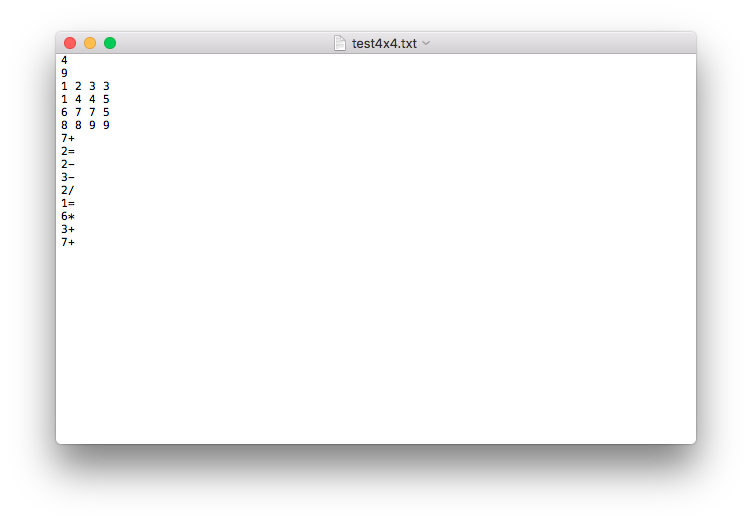
\includegraphics[scale=0.5]{Gambar/Perancangan/PerancanganInput.png}
\caption[Contoh \textit{file} masukan.]{Contoh \textit{file} masukan.}
\label{fig:perancanganmasukan}
\end{figure}

Adapun rincian dari \textit{file text} masukan tersebut adalah sebagai berikut:

\begin{enumerate}
\item Baris pertama berisi ukuran \textit{grid} dan banyaknya \textit{cage} dari teka-teki Calcudoku tersebut. Angka pertama adalah ukuran \textit{grid}, dan angka kedua adalah banyaknya \textit{cage}.
\item Baris kedua sampai ke baris ke-\begin{math}2 + (n - 1)\end{math}, dengan \begin{math}n\end{math} adalah ukuran \textit{grid}, berisi matriks \textit{cage assignment}. Matriks ini merepresentasikan posisi dari setiap \textit{cage} dalam \textit{grid}. Setiap \textit{cage} direpresentasikan dengan angka yang berbeda. Setiap \textit{cage} dapat mempunyai ukuran (jumlah sel yang terdapat dalam \textit{cage}) yang bervariasi. Setiap sel dalam sebuah \textit{cage} harus berhubungan secara horizontal atau vertikal dengan sel lain dalam \textit{cage} yang sama.
\item Baris ke-\begin{math}2 + n\end{math} dan seterusnya berisi \textit{cage objectives} untuk setiap \textit{cage}. \textit{Cage objectives} berisikan angka tujuan dan operasi matematika yang telah ditentukan. Angka-angka dalam sebuah \textit{cage} harus mencapai angka tujuan jika dihitung menggunakan operasi matematika yang telah ditentukan.
\end{enumerate}

\section{Perancangan Keluaran}
\label{sec:perancangankeluaran}

Keluaran untuk perangkat lunak permainan teka-teki Calcudoku ini berupa sebuah matriks yang berisi solusi dari teka-teki Calcudoku yang sudah diselesaikan oleh program, seperti dapat dilihat pada Gambar~\ref{fig:perancangankeluaran}.

\begin{figure}
\centering
\captionsetup{justification=centering}
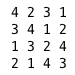
\includegraphics[scale=1]{Gambar/Perancangan/PerancanganOutput.png}
\caption[Contoh keluaran.]{Contoh keluaran.}
\label{fig:perancangankeluaran}
\end{figure}


\section{Diagram Kelas}
\label{sec:diagramkelas}

Perangkat lunak teka-teki Calcudoku ini terdiri dari beberapa kelas, yang dikelompokkan dalam tiga package, yaitu:

\begin{enumerate}
\item Model, yaitu \textit{engine} dari perangkat lunak ini. Package ini memiliki beberapa kelas, yaitu:
	\begin{enumerate}
	\item Grid, yaitu kelas yang merepresentasikan \textit{grid} dalam teka-teki Calcudoku.
	\item Cell, yaitu kelas yang merepresentasikan sel dalam teka-teki Calcudoku.
	\item Cage, yaitu kelas yang merepresentasikan \textit{cage} dalam teka-teki Calcudoku.
	\item SolverBacktracking, yaitu kelas \textit{solver} untuk teka-teki Calcudoku menggunakan algoritma backtracking.
	\item SolverHybridGenetic, yaitu kelas \textit{solver} untuk teka-teki Calcudoku menggunakan algoritma \textit{hybrid genetic}. Algoritma ini akan mencoba menyelesaikan teka-teki Calcudoku menggunakan algoritma \textit{rule based} terlebih dahulu. Algoritma genetik baru akan dijalankan jika algoritma \textit{rule based} gagal dalam menyelesaikan teka-teki Calcudoku.
	\item SolverRuleBased, yaitu kelas \textit{solver} untuk teka-teki Calcudoku menggunakan algoritma \textit{rule based}. Dalam algoritma \textit{hybrid genetic}, algoritma akan mencoba menyelesaikan teka-teki Calcudoku menggunakan algoritma \textit{rule based} terlebih dahulu.
	\item SolverGenetic, yaitu kelas \textit{solver} untuk teka-teki Calcudoku menggunakan algoritma genetik. Dalam algoritma \textit{hybrid genetic}, algoritma genetik baru akan dijalankan jika algoritma \textit{rule based} gagal dalam menyelesaikan teka-teki Calcudoku.
	\item Chromosome, yaitu kelas yang merepresentasikan sebuah kromosom untuk algoritma genetik dalam solver \textit{hybrid genetic}.
	\item ChromosomeComparator, yaitu kelas pembanding \textit{custom} (\textit{custom comparator}) yang berfungsi untuk mengurutkan kromosom berdasarkan nilai kelayakkannya (\textit{fitness value}).	
	\item SolverGenetic, yaitu kelas \textit{solver} untuk teka-teki Calcudoku menggunakan algoritma genetik. Dalam algoritma \textit{hybrid genetic}, algoritma genetik baru akan dijalankan jika algoritma \textit{rule based} gagal dalam menyelesaikan teka-teki Calcudoku.
	\end{enumerate}
\item View, yaitu tampilan dari perangkat lunak ini. Package ini memiliki beberapa kelas, yaitu:
	\begin{enumerate}
	\item Tester, yaitu kelas untuk menguji program ini.
	\end{enumerate}
\item Controller, yaitu penghubung antara package Model dan package View. Package ini hanya berisi satu kelas, yaitu kelas Controller.
\end{enumerate}

Diagram kelas untuk perangkat lunak ini dapat dilihat pada Gambar~\ref{fig:diagramkelas}.

\begin{figure}
\centering
\captionsetup{justification=centering}
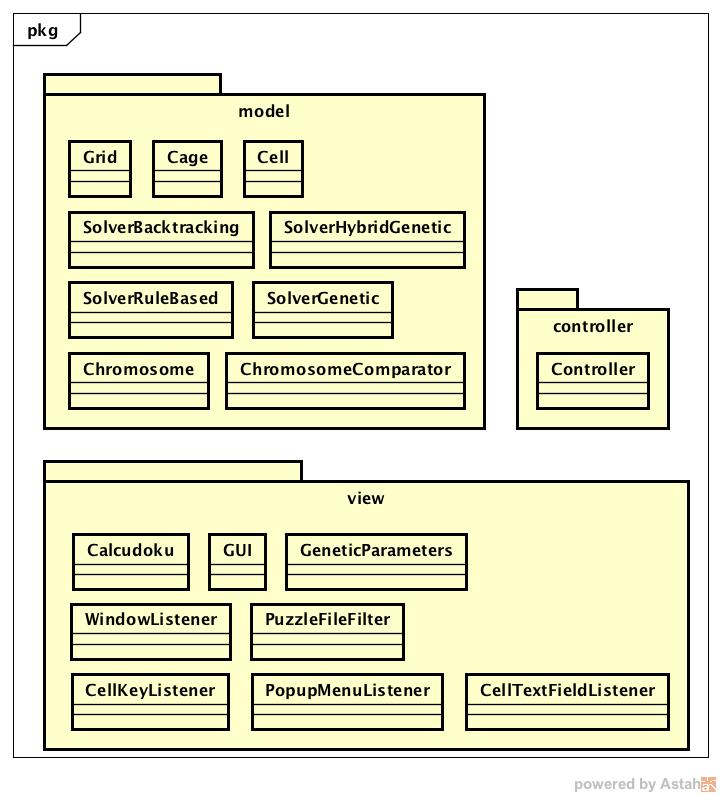
\includegraphics[scale=0.2]{Gambar/Perancangan/DiagramKelas.jpg}
\caption[Diagram kelas untuk perangkat lunak Calcudoku.]{Diagram kelas untuk perangkat lunak Calcudoku.}
\label{fig:diagramkelas}
\end{figure}

Berikut ini adalah rincian dari setiap kelas, dengan setiap atribut dan setiap \textit{method} yang dimilikinya.

\subsection{Kelas Grid}
\label{sec:kelasgrid}

Kelas Grid mempunyai beberapa atribut, yaitu:

\begin{enumerate}
\item size, yaitu ukuran dari matriks \textit{grid}.
\item numberOfCages, yaitu banyaknya \textit{cage} yang terdapat dalam \textit{grid}.
\item cageCells, yaitu sebuah matriks \textit{cage assignment}. Matriks ini merepresentasikan posisi dari setiap \textit{cage} dalam \textit{grid}.
\item cageObjectives, yaitu sebuah \textit{array} yang berisi \textit{cage objectives} untuk setiap \textit{cage}. \textit{Cage objectives} berisikan angka tujuan dan operasi matematika yang telah ditentukan.
\item grid, yaitu representasi dari \textit{grid} dalam teka-teki Calcudoku. grid adalah sebuah matriks yang berisi sel-sel. Matriks ini berukuran \begin{math} n \times n\end{math}.
\item cages, yaitu representasi dari sebuah \textit{cage} dalam sebuah \textit{grid}.
\end{enumerate}

Kelas Grid mempunyai beberapa \textit{method}, yaitu:

\begin{enumerate}
\item Grid(int size, int numberOfCages, int[][] cageCells, String[] cageObjectives), yaitu konstruktor dari kelas ini. \textit{Method} ini menerima masukan berupa ukuran dari matriks \textit{grid}, banyaknya \textit{cage} yang terdapat dalam \textit{grid}, matriks \textit{cage assignment}, dan array \textit{cage objectives}.
\item countAreas(int[][] array), yaitu \textit{method} pembungkus dari \textit{method} countAreas(int[][] array, boolean[][] checked). \textit{Method} ini menerima masukan berupa array \textit{cage assignment} untuk sebuah \textit{cage}, dan menghasilkan keluaran berupa jumlah area dari \textit{cage} tersebut.
\item countAreas(int[][] array, boolean[][] checked), yaitu \textit{method} yang menghitung jumlah area dari sebuah \textit{cage} secara rekursif dengan menggunakan algoritma \textit{flood fill}. \textit{Method} ini menerima masukan berupa array \textit{cage assignment} untuk sebuah \textit{cage} dan sebuah array checked yang berfungsi untuk menandai sel-sel yang sudah pernah dikunjungi atau belum, dan menghasilkan keluaran berupa jumlah area dari \textit{cage} tersebut.
\item floodFill(int i, int j, int[][] array, boolean[][] checked), yaitu implementasi dari algoritma \textit{flood fill} untuk menghitung jumlah area dari sebuah \textit{cage}. \textit{Method} ini menerima masukan berupa posisi baris dan kolom dari sebuah sel, array \textit{cage assignment} untuk sebuah \textit{cage} dan sebuah array checked yang berfungsi untuk menandai sel-sel yang sudah pernah dikunjungi atau belum.
\item isCageCellsSizeValid(int[][] cageCells), yaitu \textit{method} yang memeriksa apakah ukuran matriks \textit{cage assignment} valid atau tidak. \textit{Method} ini menerima masukan berupa matriks \textit{cage assignment}, dan menghasilkan keluaran apakah matriks tersebut \textit{valid} atau tidak. Matriks tersebut \textit{valid} jika ukuran barisnya dan kolomnya sama dengan variabel size.
\item isCageObjectivesSizeValid(String[] cageObjectives), yaitu \textit{method} yang memeriksa apakah ukuran matriks \textit{cage objectives} valid atau tidak. \textit{Method} ini menerima masukan berupa \textit{array cage objectives}, dan menghasilkan keluaran apakah \textit{array} tersebut \textit{valid} atau tidak. Array tersebut \textit{valid} jika ukuran dari \textit{array} tersebut sama dengan variabel numberOfCages.
\item isCageAssignmentValid(int[][] array), yaitu \textit{method} yang memeriksa apakah \textit{cage assignment} untuk sebuah \textit{cage valid} atau tidak. \textit{Method} ini menerima masukan berupa matriks \textit{cage assignment} untuk sebuah \textit{cage} dan menghasilkan keluaran apakah matriks tersebut atau tidak. Matriks tersebut \textit{valid} jika jumlah area dari \textit{cage} tersebut adalah satu.
\item isCageValid(Cage[] cages), yaitu \textit{method} yang memeriksa apakah setiap \textit{cage} yang ada di dalam \textit{grid valid} atau tidak. \textit{Method} ini menerima masukan berupa \textit{array cage}, dan menghasilkan keluaran apakah \textit{array} tersebut \textit{valid} atau tidak. \textit{Array} tersebut \textit{valid} jika setiap \textit{cage} dengan operator = hanya berukuran satu sel, setiap \textit{cage} dengan operator + atau \begin{math}\times\end{math} berukuran minimal dua sel, dan setiap \textit{cage} dengan operator - atau \begin{math}\div\end{math} berukuran tepat dua sel.
\item generateCages(Cage[] cages), yaitu \textit{method} yang membangkitkan \textit{cage-cage} dalam sebuah \textit{grid}. \textit{Method} ini menerima masukan berupa sebuah array \textit{Cage} yang kosong.
\item generateGrid(Cell[][] grid, Cage[] cages), yaitu \textit{method} yang membangkitkan \textit{grid} dan \textit{cage assignment} dari \textit{grid} tersebut.. \textit{Method} ini menerima masukan berupa sebuah matriks sel yang kosong dan sebuah array \textit{cage} yang kosong.
\item getRow(int rowNumber), yaitu \textit{method} untuk mendapatkan isi dari sebuah baris yang diminta. \textit{Method} ini menerima masukan berupa nomor baris yang diminta dan menghasilkan keluaran berupa isi baris yang diminta.
\item getColumn(int ColumnNumber), yaitu \textit{method} untuk mendapatkan isi dari sebuah kolom yang diminta. \textit{Method} ini menerima masukan berupa nomor kolom yang diminta dan menghasilkan keluaran berupa isi kolom yang diminta dalam bentuk ArrayList.
\item getCageValues(int cageNumber), yaitu \textit{method} untuk mendapatkan isi dari sebuah \textit{cage} yang diminta. \textit{Method} ini menerima masukan berupa nomor \textit{cage} yang diminta dan menghasilkan keluaran berupa isi \textit{cage} yang diminta dalam bentuk ArrayList.
\item isArrayValid(ArrayList<Integer> array), yaitu \textit{method} untuk memeriksa apakah sebuah \textit{array valid} atau tidak. \textit{Method} ini menerima masukan berupa \textit{array} yang akan diperiksa dan menghasilkan keluaran apakah \textit{array} tersebut \textit{valid} atau tidak. \textit{Array} tersebut \textit{valid} jika tidak ada angka yang berulang dalam \textit{array} tersebut.
\item isRowValid(int row), yaitu \textit{method} untuk memeriksa apakah sebuah baris \textit{valid} atau tidak. \textit{Method} ini menerima masukan berupa nomor baris yang diminta dan menghasilkan keluaran apakah baris yang diminta tersebut \textit{valid} atau tidak. Baris tersebut \textit{valid} jika tidak ada angka yang berulang dalam baris tersebut.
\item solverIsRowValid(int column), yaitu \textit{method} yang sama dengan isRowValid, tetapi \textit{method} ini hanya untuk dipanggil oleh solver.
\item isColumnValid(int column), yaitu \textit{method} untuk memeriksa apakah sebuah kolom \textit{valid} atau tidak. \textit{Method} ini menerima masukan berupa nomor kolom yang diminta dan menghasilkan keluaran apakah kolom yang diminta tersebut \textit{valid} atau tidak. Kolom tersebut \textit{valid} jika tidak ada angka yang berulang dalam kolom tersebut.
\item solverIsColumnValid(int column), yaitu \textit{method} yang sama dengan isColumnValid, tetapi \textit{method} ini hanya untuk dipanggil oleh solver.
\item isCage(int row, int column), yaitu \textit{method} untuk memeriksa apakah sebuah \textit{cage valid} atau tidak. \textit{Method} ini menerima masukan berupa nomor baris dan nomor kolom dari sebuah sel yang diminta dan menghasilkan keluaran apakah \textit{cage} yang berisi sel tersebut \textit{valid} atau tidak. \textit{Cage} tersebut \textit{valid} jika angka-angka dalam \textit{cage} tersebut mencapai angka tujuan yang telah ditentukan jika dihitung menggunakan operator yang telah ditentukan.
\item solverIsCageValid(int column), yaitu \textit{method} yang sama dengan isCageValid, tetapi \textit{method} ini hanya untuk dipanggil oleh solver.
\item isCellValueValid(int row, int column), yaitu \textit{method} untuk memeriksa apakah nilai dari sel tersebut \textit{valid} atau tidak. \textit{Method} ini menerima masukan berupa nomor baris dan nomor kolom dari sel yang akan diperiksa dan menghasilkan keluaran apakah nilai dari sel tersebut \textit{valid} atau tidak. Nilai dari sebuah sel \textit{valid} jika nilai dari sel tersebut tidak berulang dalam baris dan kolom tempat sel tersebut berada, dan angka-angka dari \textit{cage} yang berisi sel tersebut mencapai angka tujuan yang telah ditentukan jika dihitung menggunakan operator yang telah ditentukan.
\item solverIsCellValueValid(int column), yaitu \textit{method} yang sama dengan isCellValueValid, tetapi \textit{method} ini hanya untuk dipanggil oleh solver.
\item setCellValue(int row, int column, Integer value), yaitu \textit{method} untuk mengisi sebuah sel dengan nilai yang telah ditentukan. \textit{Method} ini menerima masukan berupa nomor baris dan nomor kolom dari sel yang akan diisi dan nilai dari sel tersebut, dan menghasilkan keluaran apakah nilai dari sel tersebut \textit{valid} atau tidak. Nilai dari sebuah sel \textit{valid} jika nilai dari sel tersebut tidak berulang dalam baris dan kolom tempat sel tersebut berada, dan angka-angka dari \textit{cage} yang berisi sel tersebut mencapai angka tujuan yang telah ditentukan jika dihitung menggunakan operator yang telah ditentukan.
\item solverSetCellValue(int row, int column, Integer value), yaitu \textit{method} yang sama dengan setCellValue, tetapi \textit{method} ini hanya untuk dipanggil oleh solver.
\item unsetCellVaue(int row, int column), yaitu metho duntuk menghapus isi dari sebuah sel. \textit{Method} ini menerima masukan berupa nomor baris dan nomor kolom dari sel yang akan dihapus isinya.
\item isWin(), yaitu \textit{method} yang memeriksa apakah semua sel sudah diisi dengan nilai yang \textit{valid} atau tidak. \textit{Method} ini menghasilkan keluaran apakah semua sel sudah diisi dengan yang \textit{valid} atau tidak. \textit{Method} ini menghasilkan \textit{null} jika ada sel yang belum diisi.
\item isFilled(), yaitu \textit{method} yang memeriksa apakah semua sel sudah diisi atau tidak. \textit{Method} ini menghasilkan keluaran apakah semua sel sudah diisi atau tidak.
\item getCellValue(int row, int column), yaitu \textit{method} untuk mendapatkan isi dari sebuah sel. \textit{Method} ini menerima masukan berupa nomor baris dan nomor kolom dari sel yang diminta dan menghasilkan keluaran berupa isi dari sel yang diminta tersebut.
\item getSize(), yaitu \textit{method} untuk mendapatkan ukuran dari \textit{grid}. \textit{Method} ini menghasilkan keluaran berupa ukuran dari \textit{grid}.
\item getCageCells(), yaitu \textit{method} untuk mendapatkan matriks \textit{cage assignment} dari \textit{grid}. \textit{Method} ini menghasilkan keluaran berupa matriks \textit{cage assignment} dari \textit{grid}.
\item getCageObjectives(), yaitu \textit{method} untuk mendapatkan \textit{cage objectives} dari setiap \textit{cage} dalam \textit{grid}. \textit{Method} ini menghasilkan keluaran berupa sebuah array yang berisi \textit{cage objectives} dari setiap \textit{cage} dalam \textit{grid}.
\item getGridContents(), yaitu \textit{method} untuk mendapatkan nilai dari setiap sel \textit{grid}. \textit{Method} ini menghasilkan keluaran berupa sebuah matriks yang berisi nilai dari setiap sel \textit{grid}.
\item getCage(), yaitu \textit{method} untuk mendapatkan semua \textit{cage} dalam \textit{grid}. \textit{Method} ini menghasilkan keluaran berupa array yang berisi semua \textit{cage} dalam \textit{grid}.
\item solveBacktracking(), yaitu \textit{method} untuk memanggil solver untuk menyelesaikan teka-teki Calcudoku menggunakan algoritma \textit{backtracking}. 
\item solveHybridGenetic(), yaitu \textit{method} untuk memanggil solver untuk menyelesaikan teka-teki Calcudoku menggunakan algoritma \textit{hybrid genetic}. 
\end{enumerate}

Diagram kelas Grid dapat dilihat pada Gambar~\ref{fig:diagramkelasgrid}.

\begin{figure}
\centering
\captionsetup{justification=centering}
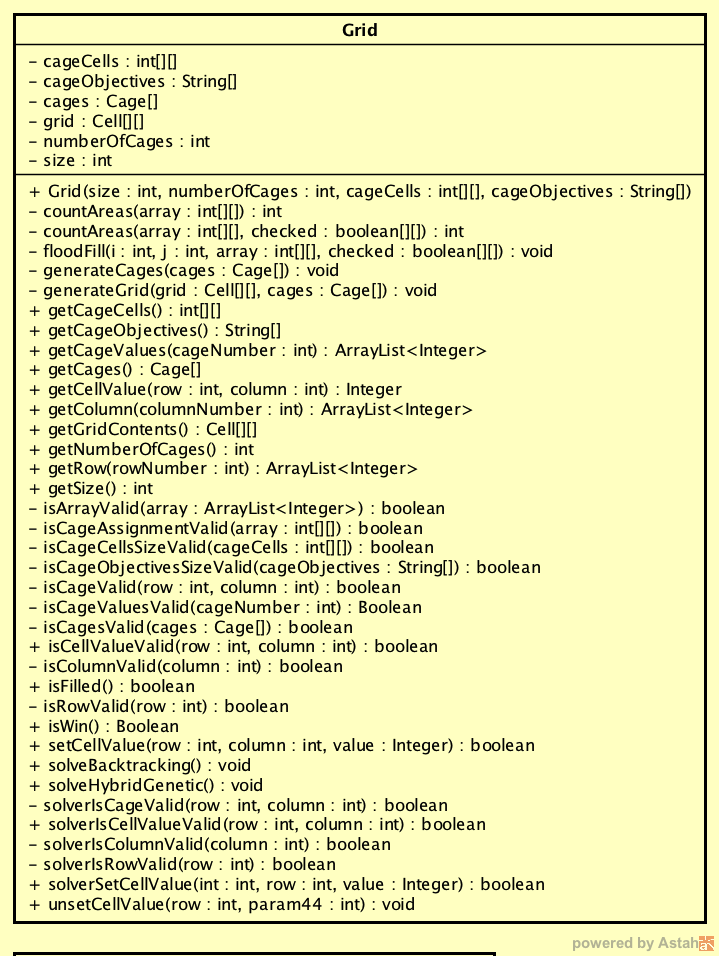
\includegraphics[scale=0.5]{Gambar/Perancangan/DiagramKelasGrid.png}
\caption[Diagram kelas Grid.]{Diagram kelas Grid.}
\label{fig:diagramkelasgrid}
\end{figure}

\subsection{Kelas Cage}
\label{sec:kelascage}

Kelas Cage mempunyai beberapa atribut, yaitu:

\begin{enumerate}
\item cageID, yaitu nomor dari \textit{cage} tersebut.
\item objective, yaitu angka tujuan dan operator yang ditentukan untuk \textit{cage} tersebut.
\item targetNumber, yaitu angka tujuan dari \textit{cage} tersebut.
\item operator, yaitu operator yang ditentukan untuk \textit{cage} tersebut.
\item cells, yaitu sebuah array yang berisi sel-sel yang merupakan anggota dari \textit{cage} tersebut.
\end{enumerate}

Kelas Cage mempunyai beberapa \textit{method}, yaitu:

\begin{enumerate}
\item Cage(int cageID, String objectives), yaitu konstruktor dari kelas ini. \textit{Method} ini menerima masukan berupa nomor dan \textit{cage objectives} dari \textit{cage} tersebut.
\item isCageObjectiveValid(String cageObjective), yaitu \textit{method} yang memeriksa apakah \textit{cage objective} dari \textit{cage} tersebut \textit{valid} atau tidak. \textit{Method} ini menerima masukan berupa String yang berisi \textit{cage objective} dan menghasilkan keluaran apakah String tersebut valid atau tidak. \textit{Cage objective valid} jika isi dari \textit{cage objective} tersebut adalah satu angka tujuan dari \textit{cage} tersebut dan diikuti oleh satu operator yang telah ditentukan untuk \textit{cage} tersebut.
\item generateTargetNumber(String objective), yaitu \textit{method} yang membangkitkan angka tujuan dari sebuah \textit{cage} dari \textit{cage objective} yang diberikan. \textit{Method} ini menerima masukan berupa String yang berisi \textit{cage objective} dari sebuah \textit{cage} dan menghasilkan keluaran berupa angka tujuan dari \textit{cage} tersebut.
\item generateOperator(String objective), yaitu \textit{method} yang membangkitkan operator yang telah ditentukan untuk sebuah \textit{cage} dari \textit{cage objective} yang diberikan. \textit{Method} ini menerima masukan berupa String yang berisi \textit{cage objective} dari sebuah \textit{cage} dan menghasilkan keluaran berupa operator yang telah ditentukan untuk \textit{cage} tersebut.
\item addCell(Cell c), yaitu \textit{method} untuk menambahkan sebuah sel kedalam sebuah \textit{cage}. \textit{Method} ini menerima masukan berupa sel yang akan dimasukkan ke dalam \textit{cage}.
\item isCageContainsNull(), yaitu \textit{method} yang memeriksa apakah sebuah \textit{cage} mempunyai sel yang belum diisi. \textit{Method} ini menghasilkan keluaran apakah \textit{cage} tersebut mempunyai sel yang belum terisi.
\item isCageValid(), yaitu \textit{method} yang memeriksa apakah angka-angka dalam sebuah \textit{cage} mencapai angka tujuan dari \textit{cage} tersebut jika dihitung menggunakan operator yang telah ditentukan untuk \textit{cage} tersebut. \textit{Method} ini menghasilkan keluaran apakah angka-angka dalam \textit{cage} tersebut mencapai angka tujuan dari \textit{cage} tersebut jika dihitung menggunakan operator yang telah ditentukan untuk \textit{cage} tersebut. \textit{Method} ini menghasilkan \textit{null} jika ada sel di dalam \textit{cage} yang belum diisi.
\item countValue(), yaitu \textit{method} yang menghitung angka-angka di dalam sebuah \textit{cage} menggunakan operator yang telah ditentukan untuk \textit{cage} tersebut. \textit{Method} ini menghasilkan keluaran hasil perhitungan dari angka-angka di dalam sebuah \textit{cage} menggunakan operator yang telah ditentukan untuk \textit{cage} tersebut. \textit{Method} ini menghasilkan \textit{null} jika ada sel di dalam \textit{cage} yang belum diisi.
\item getTargetNumber(), yaitu \textit{method} untuk mendapatkan angka tujuan dari sebuah \textit{cage}. \textit{Method} ini menghasilkan keluaran berupa angka tujuan dari \textit{cage} tersebut.
\item getTargetNumber(), yaitu \textit{method} untuk mendapatkan operator yang telah ditentukan untuk sebuah \textit{cage}. \textit{Method} ini menghasilkan keluaran berupa operator yang telah ditentukan untuk \textit{cage} tersebut.
\item getCells(), yaitu \textit{method} untuk mendapatkan sel-sel anggota sebuah \textit{cage}. \textit{Method} ini menghasilkan keluaran sebuah ArrayList yang berisi sel-sel anggota \textit{cage} tersebut.
\item getSize(), yaitu \textit{method} untuk mendapatkan jumlah dari sel-sel anggota sebuah \textit{cage}. \textit{Method} ini menghasilkan keluaran berupa jumlah dari sel-sel anggota \textit{cage} tersebut.
\end{enumerate}

Diagram kelas Cage dapat dilihat pada Gambar~\ref{fig:diagramkelascage}.

\begin{figure}
\centering
\captionsetup{justification=centering}
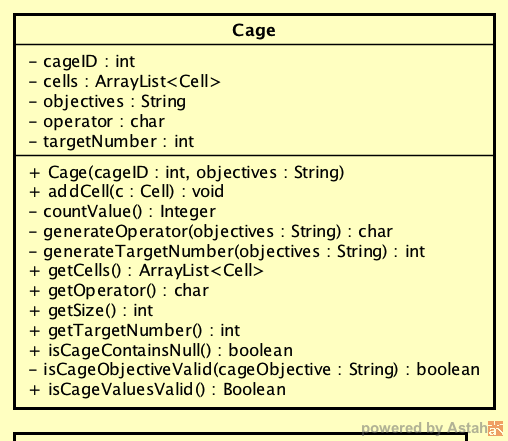
\includegraphics[scale=0.5]{Gambar/Perancangan/DiagramKelasCage.png}
\caption[Diagram kelas Cage.]{Diagram kelas Cage.}
\label{fig:diagramkelascage}
\end{figure}

\subsection{Kelas Cell}
\label{sec:kelascell}

Kelas Cell mempunyai beberapa atribut, yaitu:

\begin{enumerate}
\item cellID, yaitu nomor dari sel tersebut.
\item row, yaitu posisi baris dari sel tersebut.
\item column, yaitu posisi kolom dari sel tersebut.
\item cageID, yaitu nomor \textit{cage} yang berisi sel tersebut.
\item value, yaitu nilai dari sel tersebut.
\end{enumerate}

Kelas Cell mempunyai beberapa \textit{method}, yaitu:

\begin{enumerate}
\item Cell(int CellID, int row, int column, int cageID), yaitu konstruktor dari kelas ini. \textit{Method} ini menerima masukan berupa nomor sel, nomor baris, dan nomor kolom dari sel tersebut, dan nomor \textit{cage} yang berisi sel tersebut.
\item setValue(Integer value), yaitu \textit{method} untuk mengisi sebuah sel tersebut dengan nilai yang telah ditentukan. \textit{Method} ini menerima masukan berupa nilai yang akan diisikan ke dalam sel tersebut.
\item getRow(), yaitu \textit{method} untuk mendapatkan nomor baris dari sebuah sel. \textit{Method} ini menghasilkan keluaran berupa nomor baris dari sel tersebut.
\item getColumn(), yaitu \textit{method} untuk mendapatkan nomor kolom dari sebuah sel. \textit{Method} ini menghasilkan keluaran berupa nomor kolom dari sel tersebut.
\item getCageID(), yaitu \textit{method} untuk mendapatkan nomor \textit{cage} yang berisi sebuah sel. \textit{Method} ini menghasilkan keluaran berupa nomor \textit{cage} yang berisi sel tersebut.
\item getCageID(), yaitu \textit{method} untuk mendapatkan nomor sel dari sebuah sel. \textit{Method} ini menghasilkan keluaran berupa nomor sel dari sel tersebut.
\end{enumerate}

Diagram kelas Cell dapat dilihat pada Gambar~\ref{fig:diagramkelascell}.

\begin{figure}
\centering
\captionsetup{justification=centering}
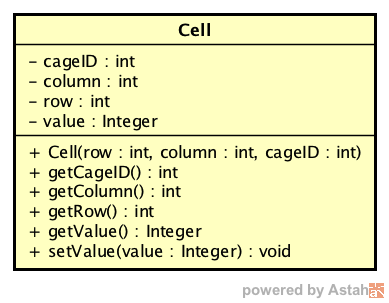
\includegraphics[scale=0.5]{Gambar/Perancangan/DiagramKelasCell.png}
\caption[Diagram kelas Cell.]{Diagram kelas Cell.}
\label{fig:diagramkelascell}
\end{figure}

\subsection{Kelas SolverBacktracking}
\label{sec:kelasbacktracking}

Kelas SolverBacktracking mempunyai beberapa atribut, yaitu:

\begin{enumerate}
\item grid, yaitu \textit{grid} yang akan diselesaikan oleh \textit{solver} dengan algoritma \textit{backtracking}.
\item size, yaitu ukuran dari \textit{grid} yang akan diselesaikan oleh \textit{solver} dengan algoritma \textit{backtracking}.
\item solution, yaitu \textit{grid} yang sudah diselesaikan oleh \textit{solver} dengan algoritma \textit{backtracking}.
\end{enumerate}

Kelas SolverBacktracking mempunyai beberapa \textit{method}, yaitu:

\begin{enumerate}
\item SolverBacktracking(Grid grid), yaitu konstruktor dari kelas ini. \textit{Method} ini menerima masukan berupa \textit{grid} yang akan diselesaikan oleh \textit{solver} dengan algoritma \textit{backtracking}.
\item solve(), yaitu \textit{method} pembungkus dari \textit{method} solve(int row, int column). Method ini menghasilkan keluaran apakah \textit{solver} berhasil menyelesaikan teka-teki Calcudoku atau tidak. \textit{Solver} bekerja mulai dari sel pada sudut kiri atas, lalu bergerak ke kanan sampai ke sel yang paling kanan, lalu bergerak ke baris berikutnya sampai ke baris yang paling bawah, selesai pada sel pada sudut kanan bawah.
\item solve(int row, int column), yaitu \textit{method} yang mencoba untuk menyelesaikan teka-teki Calcudoku. Method ini menerima masukan berupa nomor baris dan nomor kolom yang akan diisi oleh \textit{solver} dan menghasilkan keluaran apakah nilai yang diisi oleh \textit{solver valid} atau tidak. \textit{Solver} akan mulai mengisi sel dari angka 1. Jika berhasil, maka \textit{solver} akan maju ke sel berikutnya. Jika gagal, maka \textit{solver} akan mencoba kemungkinan angka berikutnya. Jika semua kemungkinan angka gagal, maka \textit{solver} akan mundur ke sel sebelumnya dan mencoba kemungkinan angka berikutnya.
\item getGrid(), yaitu \textit{method} untuk mendapatkan \textit{grid}. Method ini menghasilkan keluaran berupa \textit{grid}.
\item getSolution(), yaitu \textit{method} untuk mendapatkan solusi dari \textit{grid} yang sudah diselesaikan oleh \textit{solver}. \textit{Method} ini menghasilkan keluaran berupa solusi dari \textit{grid} tersebut.
\item printGrid(), yaitu \textit{method} untuk mencetak isi \textit{grid} ke layar.
\end{enumerate}

Diagram kelas SolverBacktracking dapat dilihat pada Gambar~\ref{fig:diagramkelassolverbt}.

\begin{figure}
\centering
\captionsetup{justification=centering}
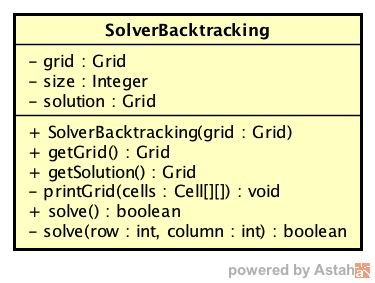
\includegraphics[scale=0.5]{Gambar/Perancangan/DiagramKelasSolverBacktracking.png}
\caption[Diagram kelas SolverBacktracking.]{Diagram kelas SolverBacktracking.}
\label{fig:diagramkelassolverbt}
\end{figure}